\documentclass{egpubl}
\usepackage{EGVMV14}

% --- for  Annual CONFERENCE
% \ConferenceSubmission % uncomment for Conference submission
% \ConferencePaper      % uncomment for (final) Conference Paper
% \STAR                 % uncomment for STAR contribution
% \Tutorial             % uncomment for Tutorial contribution
% \ShortPresentation    % uncomment for (final) Short Conference Presentation
%
% --- for  CGF Journal
% \JournalSubmission    % uncomment for submission to Computer Graphics Forum
% \JournalPaper         % uncomment for final version of Journal Paper
%
% --- for  CGF Journal: special issue
% \SpecialIssueSubmission    % uncomment for submission to Computer Graphics Forum, special issue
% \SpecialIssuePaper         % uncomment for final version of Journal Paper, special issue
%
% --- for  EG Workshop Proceedings
 \WsSubmission    % uncomment for submission to EG Workshop
% \WsPaper         % uncomment for final version of EG Workshop contribution
%
 \electronicVersion % can be used both for the printed and electronic version

% !! *please* don't change anything above
% !! unless you REALLY know what you are doing
% ------------------------------------------------------------------------

% for including postscript figures
% mind: package option 'draft' will replace PS figure by a filname within a frame
\ifpdf \usepackage[pdftex]{graphicx} \pdfcompresslevel=9
\else \usepackage[dvips]{graphicx} \fi

\PrintedOrElectronic

% prepare for electronic version of your document
\usepackage{t1enc,dfadobe}
\usepackage{url}
\usepackage{mathptmx}
\usepackage{graphicx}
\usepackage{times}
\usepackage[usenames,dvipsnames,svgnames]{xcolor}
\usepackage{subfigure}
\usepackage{flushend}
\usepackage[compact]{titlesec}
\usepackage[normalem]{ulem}

\usepackage{egweblnk}
\usepackage{cite}

%\usepackage[bookmarks,backref=true,linkcolor=black]{hyperref} %,colorlinks
%\hypersetup{
%  pdfauthor = {},
%  pdftitle = {},
%  pdfsubject = {},
%  pdfkeywords = {},
%  colorlinks=true,
%  linkcolor= black,
%  citecolor= black,
%  pageanchor=true,
%  urlcolor = black,
%  plainpages = false,
%  linktocpage
%}

% For backwards compatibility to old LaTeX type font selection.
% Uncomment if your document adheres to LaTeX2e recommendations.
\let\rm=\rmfamily    \let\sf=\sffamily    \let\tt=\ttfamily
\let\it=\itshape     \let\sl=\slshape     \let\sc=\scshape
\let\bf=\bfseries

\def\etal{\textit{et al.}}
\definecolor{MyGreen}{rgb}{0,0.7,0}
\definecolor{MyWhite}{rgb}{1,1,1}
\definecolor{MyGray}{rgb}{0.5,0.5,0.5}
\definecolor{LightGray}{rgb}{0.7,0.7,0.7}
\definecolor{DarkGray}{rgb}{0.3,0.3,0.3}
\definecolor{DarkYellow}{rgb}{0.7,0.7,0.0}
\definecolor{MyNavyBlue}{rgb}{0.2,0.3,0.7}
\definecolor{darkgreen}{rgb}{0,0.55,0}
\newcommand{\black}[1]{{\color{Black} #1}}
\newcommand{\white}[1]{{\color{MyWhite} #1}}
\newcommand{\gray}[1]{{\color{MyGray} #1}}
\newcommand{\red}[1]{{\color{red} #1}}
\newcommand{\green}[1]{{\color{MyGreen} #1}}
\newcommand{\blue}[1]{{\color{MyNavyBlue} #1}}
\newcommand{\yellow}[1]{{\color{DarkYellow} #1}}
\newcommand{\maybe}[1]{\yellow{#1}}
\newcommand{\rout}[1]{\red{\sout{#1}}}
\newcommand{\repl}[2]{\rout{#1} \green{#2}}
\newcommand{\fix}[1]{\red{\emph{(#1)}}}
\newcommand{\Fix}[1]{\begin{itemize} \renewcommand\labelitemi{\red{--}} \item \red{#1} 
\end{itemize}}

\newcommand{\todo}[1] {\textbf{[~}\textcolor {red}{#1}\marginpar{\textcolor {red}{\centerline{{\Huge \textbf{!}}}}}\textbf{~]}}
\newcommand{\question}[1] {\textbf{[~}\textcolor {darkgreen}{#1}\marginpar{\textcolor {darkgreen}{\centerline{{\Huge \textbf{!}}}}}\textbf{~]}}
\newcommand{\diff}[1]{[\textcolor{blue}{#1}\marginpar{\textcolor{blue}{\centerline{{\Huge \textbf{!}}}}}]}

\def\IC{IC}
\def\SAR{SAR}
\def\USAR{USAR}

\setlength\fboxsep{0pt}

% end of prologue


%% Paper title.
%\title[Decision-Support for Search \& Rescue Planning]{Decision-Support for Urban Search \& Rescue Mission Planning through Visualization-Based Analysis}
\title[Urban Search \& Rescue Mission Planning]{Supporting Urban Search \& Rescue Mission Planning\\ through Visualization-Based Analysis}

\author[Bock \etal]{
    Alexander Bock$^1$, Alexander Kleiner$^2$, Jonas Lundberg$^3$, and Timo Ropinski$^1$\\%
    $^1$Scientific Visualization Group, Link\"oping University\\%
    $^2$Collaborative Robotics Group, Link\"oping University\\%
    {\small $^3$Graphic Design Group, Link\"oping University}
}   

%\authorfooter{
%    \item Alexander Bock and Timo Ropinski are with the Scientific Visualization Group, Link\"oping University. e-mail: \{alexander.bock\textbar timo.ropinski\}@liu.se
%    \item Jonas Lundberg is with the Graphic Design Group, Link\"oping University. e-mail: jonas.lundberg@liu.se
%    \item Alexander Kleiner is with the Collaborative Robotics Group, Link\"oping University. e-mail: alexander.kleiner@liu.se
%}

%\shortauthortitle{Bock \etal: Urban Search \& Rescue Mission Planning}

%% Keywords that describe your work. Will show as 'Index Terms' in journal
%% please capitalize first letter and insert punctuation after last keyword
%\keywords{Urban search~\&~rescue mission planning, decision support, visual analysis.}

%% ACM Computing Classification System (CCS). 
%% See <http://www.acm.org/class/1998/> for details.
%% The ``\CCScat'' command takes four arguments.


%% Uncomment below to disable the manuscript note
%\renewcommand{\manuscriptnotetxt}{}

%% Copyright space is enabled by default as required by guidelines.
%% It is disabled by the 'review' option or via the following command:
% \nocopyrightspace

%%%%%%%%%%%%%%%%%%%%%%%%%%%%%%%%%%%%%%%%%%%%%%%%%%%%%%%%%%%%%%%%%%%%%%%%%%%%%%%%%%%%%%%%%%%
%%%%%%%%%%%%%%%%%%%%%%%%%%%%%%%%%%%%%%%%%%%%%%%%%%%%%%%%%%%%%%%%%%%%%%%%%%%%%%%%%%%%%%%%%%%

\begin{document}

\teaser{
	\centering
	\subfigure[Voxelized 3D point cloud rendering enabling an increased awareness of a damaged office building.]{
		\fbox{\includegraphics[height=0.26\linewidth]{figures/image1.jpg}}\label{fig:teaser:1}
	}
	\hfill
	\subfigure[Viable paths through buildings of the Tohoku university with two hazardous environments highlighted.]{
		\fbox{\includegraphics[height=0.26\linewidth]{figures/image2.jpg}}\label{fig:teaser:2}
	}
	\hfill
	\subfigure[Top-down view of the area providing contextual information.]{
		\fbox{\includegraphics[height=0.26\linewidth]{figures/image2-overview.jpg}}\label{fig:teaser:3}
	}
	\hfill
	\subfigure[Analysis of a path ensemble using parallel coordinates plots and profile plots.]{
		\fbox{\includegraphics[height=0.26\linewidth]{figures/pcpprofile.png}}\label{fig:teaser:4}
	}
  \caption{Our proposed visualization system applied to path planning in a collapsed building at Tohoku university. Different views (a--c) present the operator with an understanding of the building, allowing him to select and inspect paths that reach a point of interest. The assessment of the trade-off between paths is supported by a set of interactive visual analysis tools (d).}
  \label{fig:teaser}
}

\maketitle

\begin{abstract}
We propose a visualization system for incident commanders in urban search~\&~rescue scenarios that supports access path planning for post-disaster structures. Utilizing point cloud data acquired from unmanned robots, we provide methods for assessment of automatically generated paths. As data uncertainty and a priori unknown information make fully automated systems impractical, we present a set of viable access paths, based on varying risk factors, in a 3D environment combined with the visual analysis tools enabling informed decisions and trade-offs. Based on these decisions, a responder is guided along the path by the incident commander, who can interactively annotate and reevaluate the acquired point cloud to react to the dynamics of the situation. We describe design considerations for our system, technical realizations, and discuss the results of an expert evaluation.

\begin{classification}
   \CCScat{I.3.7}{Computer Graphics}{Three-Dimensional Graphics and Realism}{Color, shading, shadowing, and texture}
\end{classification}


\end{abstract}

\section{Introduction}

Natural disasters causing structural damage to inhabited buildings are an ever-present danger. As time-to-rescue is one of the most important factors determining victims' survivability, it is of highest importance for rescue responders to reach victims as fast as possible in order to provide medical attention or extraction. Planning and executing paths through buildings, however, is difficult due to structural damages making available floor plans outdated. Furthermore, structural weaknesses as well as hazardous environments, make regions and areas inaccessible. While trained responders can use their knowledge and intuition to spot these hazards, it is paramount that the \emph{Incident Commander} (IC) can analyze the information and coordinate multiple rescue responders. In order to design a computer support system that amplifies human decision-making, it is vital to consider how decisions in dynamic situations are made~\cite{Lundberg2012}. The system is then designed to support planning based on experience, to increase quality of control, and to support decision-making, not only with regard to expected decisions, but also considering unexpected developments.

There exist well-defined protocols describing the actions taken during an \emph{Urban Search~\&~Rescue} (USAR) operation. The Federal Emergency Management Agency describes five steps that are performed by the rescue team~\cite{fema08}. During the assessment step, 2D maps of the collapsed building are drawn based on the descriptions of rescue responders moving about the building searching for victims. In this exploration phase, they might stumble into hazardous areas that endanger the rescuer's life.

In recent years, technological developments made it possible to use unmanned vehicles to perform the initial exploration. The robots can be deployed into the building and are equipped with sensors that can detect victims, gather information about potentially hazardous environments, and perform detailed scans of rooms to create a 3D point cloud of the interior. After the map has been acquired, the \IC\ can analyze the collected data and plan viable access paths entering the building to reach certain \emph{Points of Interest} (POIs). In most cases, these POIs are potential locations of victims, but they can also be other mission critical areas that need to be reached and analyzed.

In this paper, we propose a visualization system that creates an interactive 3D rendering tailored to increase the \IC 's awareness of internal structures (see Figure~\ref{fig:teaser}~(a-c)) and supporting the analysis and planning of access paths (see Figure~\ref{fig:teaser}~(d)). The \IC\ can annotate the visualization with real-time information from on-site rescue responders, thus shifting the opportunistic decision making to being strategical. Our system computes an ensemble of access paths from the entry point to the POIs, where each path is based on varying risk factors. Uncertainty in the data and a priori unknown information make it infeasible to employ automatic algorithms to detect the globally optimal path. Our system supports the \IC\ in the process of analyzing and comparing all available paths at once to minimize the rescuer's danger and travel time.

%%%%%%%%%%%%%%%%%%%%%%%%%%%%%%%%%%%%%%%%%%%%%%%%%%%%%%%%%%%%%%%%%%%%%%%%%%%%%%%%%%%%%%%%%%%
%%%%%%%%%%%%%%%%%%%%%%%%%%%%%%%%%%%%%%%%%%%%%%%%%%%%%%%%%%%%%%%%%%%%%%%%%%%%%%%%%%%%%%%%%%%

\section{Related Work} \label{sec:relatedwork}
\noindent {\bfseries Emergency management.} Much of the visualization-oriented work published in the field of emergency management is concerned with evacuation planning well before any rescue operation has to be performed. Notable work was performed by Reddy~\etal, which enables analyzing possible bottlenecks of escape routes~\cite{EuroVA12:13-17:2012}. Ribarsky~\etal\ presented a system organizing first responders in intact structures~\cite{Ribarsky:2010}. Kim~\etal\ developed a system enhancing the situational awareness of responders using a mobile visual analytics tool~\cite{Kim:2008}.

Many existing planning systems deployed nowadays in USAR scenarios are based on 2D representations~\cite{kleiner_et_al_ssrr09,KohlbrecherMeyerStrykKlingaufFlexibleSlamSystem2011,Pellenz2009SMU}. Given the 2D map of the environment, one common approach to path planning is to plan the shortest trajectory and to follow this trajectory stepwise. In harsh environments, however, the safest path, not the shortest, may be desirable. Wirth~\etal\ introduced an exploration strategy and path planner that utilizes occupancy grid maps when planning to reach several targets at the same time~\cite{Wirth2007ETA1}. Preliminary extensions towards exploration in 3D with regard to detection of voids were introduced by Dornhege and Kleiner~\cite{dornhege2011frontier}.

\noindent {\bfseries Point cloud visualization.} As the availability of point cloud data increased in recent years, there has been much research on rendering techniques for this kind of data. Basic rendering capabilities are provided by the widely used Point Cloud Library~\cite{Rusu11ICRA}. Furthermore, work by Richter~\etal\ uses a level-of-detail structure to render massive point clouds at high frame rates~\cite{Richter:2010:ORV:1811158.1811178}. More recently, Pintus~\etal\ presented a rendering algorithm that enhances features of unstructured point clouds without preprocessing~\cite{Pintus:2011:RRM:2384495.2384513}.

%%%%%%%%%%%%%%%%%%%%%%%%%%%%%%%%%%%%%%%%%%%%%%%%%%%%%%%%%%%%%%%%%%%%%%%%%%%%%%%%%%%%%%%%%%%
%%%%%%%%%%%%%%%%%%%%%%%%%%%%%%%%%%%%%%%%%%%%%%%%%%%%%%%%%%%%%%%%%%%%%%%%%%%%%%%%%%%%%%%%%%%

\section{Decision-Making Theory} \label{sec:theory}
To be able to design a decision support system for USAR missions, it is crucial to take knowledge about human decision making into account. Human decision makers tend to evaluate options serially in time-constrained situations. They attempt to find one viable plan that should work rather than attempting to generate and compare numerous plans in parallel. This theory has been described by Klein and Calderwood as \emph{Recognition Primed Decision-making} (RPD)~\cite{KleinCalderwood}. Initially, human experts look for similarities to previous situations with regard to relevant goals, things that were important to monitor, and possible actions. Then, they go through a process of mental simulation to consider whether the actions are applicable to the case at hand. They assess the ongoing situation, looking for violations and confirmations of expectancies, which may require reframing the situation. Klein and Calderwood suggest that ``displays and interfaces can be centered on decisions rather than around data flows''~\cite{KleinCalderwood}, emphasizing that systems can be built to enhance the workflow of mental simulation. 

The \emph{Contextual Control Model} (COCOM) by Hollnagel and Woods describes how people rely on context when making decisions~\cite{hollnagel2005joint}. This theory recognizes that humans sometimes act with plans of lower quality, relying on the environment to make decisions opportunistically without having a  plan to reach the goal. The quality of their control of the situation can be described as scrambled, opportunistic, tactical, or strategic. The scrambled mode refers to decisions made without any idea of what to do. In the opportunistic mode, people rely on cues in the local context to decide on their next action. In tactical mode, they have an idea of how to achieve their goal before taking action---a plan. In strategic mode, the plan includes coordination with other simultaneous goals. The goal of our proposed system is to raise the quality of control from being opportunistic (as in the current workflow) to being strategic, thus enabling improved decision-making capabilities.

Turning to the granularity of plans, the \emph{Extended Control Model} (ECOM) describes plans in terms of a tactical level (setting goals), monitoring (making plans and overseeing plans), regulating (managing local resources), and tracking (performing and adjusting actions)~\cite{hollnagel2005joint}. This theory can be used to apprise what kind of planning support a system provides.  Moreover, it has been argued by Lundberg~\etal\ that it is important to support resiliency: ``Rather than merely selecting a response from a ready-made table, [the system] must adapt and create a suitable response; either by following ready-made plans for adaptation or by making sense of the situation and create responses during the unfolding event''~\cite{Lundberg2012}. Thus, in addition to supporting specific responses that may be foreseen, the system should also support working outside of prepared situations.

%%%%%%%%%%%%%%%%%%%%%%%%%%%%%%%%%%%%%%%%%%%%%%%%%%%%%%%%%%%%%%%%%%%%%%%%%%%%%%%%%%%%%%%%%%%
%%%%%%%%%%%%%%%%%%%%%%%%%%%%%%%%%%%%%%%%%%%%%%%%%%%%%%%%%%%%%%%%%%%%%%%%%%%%%%%%%%%%%%%%%%%

\section{Incident Commander Workflow} \label{sec:workflow}

\begin{figure}
	\centering
	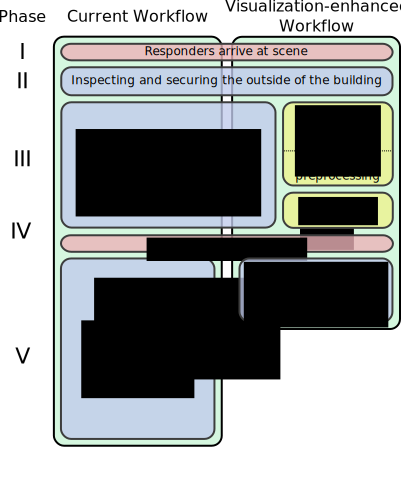
\includegraphics[width=0.9\columnwidth]{figures/workflow.pdf}
	\caption{A schematic timeline overview of the currently employed workflow (left) and our proposed system (right), showing all events (red) and actions (blue) split up into five distinct phases. Utilizing the additional actions (yellow) in parallel and thus enabling faster exploration, we decrease the overall time-to-rescue.}
	\label{fig:workflow:workflow}
\end{figure}

While there is no general definition of a rescue team in an USAR incident, in most protocols, for example in FEMA~\cite{fema08} or Emergency Management Australia~\cite{em35}, one \IC\ is responsible for a single building and instructs multiple rescue responders inside. In this section, we will describe the current workflow first (see Figure~\ref{fig:workflow:workflow}, left) and then propose a visualization-enhanced workflow supported by our system (see Figure~\ref{fig:workflow:workflow}, right). Roman numerals in the text refer to the corresponding phases in the figure.

\noindent {\bfseries Current workflow.} After arriving at the disaster scene (Phase \texttt{I}), the first step for the responders is to explore and secure the area outside the collapsed building (Phase \texttt{II}). No rescuer is allowed to enter the building before it is secured, which can take an hour or more to finish (Phase \texttt{III}). Then, the \IC\ determines entry points into the structure and directs rescuers to perform reconnaissance (Phase \texttt{IV}). Using constant radio communication, the rescuer inside the building slowly advances and reports his progress to the \IC, who draws a 2D map (see Figure~\ref{fig:workflow:sota}) (Phase \texttt{V}). This exposes the rescuer to unquantifiable risks, like gas leaks or dormant fires. This is clearly an example of opportunistic control, where decisions are made opportunistically based on feedback from the environment. Although responders may recognize situations, decisions regarding the path are limited to the extent of the exploration and to their view of the local environment. Global planning is limited further by the ability of responders to communicate relevant structural information accurately to the \IC, such as angles of turns, which cause hand-drawn maps to experience drift.

\noindent {\bfseries Visualization-enhanced workflow.} The initial phases \texttt{I} and \texttt{II} are the same as in the workflow above. However, while the responders secure the building, the most time-consuming of the initial tasks, unmanned robots are released into the structure and start measuring the inside of the structure~(see the parallel execution in phase \texttt{III}). The robots' sensors are able to detect many signs of victims using thermal cameras and heart beat detectors~\cite{6027084, Wu12Eulerian}, but as these measurements are uncertain, false positives and false negatives might occur. The same holds true for hazardous environments like fires, gas leaks, structurally unsafe areas, chemical spills, or radiation. The data retrieval and preprocessing are done in parallel with securing the perimeter, so that all information is available without delay when phase \texttt{IV} begins. Based on suggested POIs, the system computes optimal paths through the generated map. This reduces time-to-rescue (Phase \texttt{V}) as the rescuers do not need to explore the building to the same extent. The proposed system applies RPD to the whole situation and extends the number of available planning from local conditions to higher ECOM levels.

When planning the access paths, a variety of factors must be taken into account. The responder must maintain a safe distance from hazardous environments, avoid overhanging structures, and the ground must be both stable and level. As these variables are extracted from uncertain data, they are difficult to quantify and are subject to uncertainties. The \IC\ has to perform trade-offs to choose between alternatives, for example favoring a longer path that is faster to traverse over a more dangerous, shorter path. These requirements make the path selection a perfect example demonstrating how the human-in-the-loop paradigm benefits the decision-making.

While the \IC\ is instructing the rescuer to follow one path, the rescuer feeds back information about possible victims or new hazards. The \IC\ incorporates this information into the system. This is of high importance as features might not only have been missed by the robots, but detected features might change during the rescue operation. Fires can start or extinguish, subsequent structural collapses can make areas inaccessible, or debris is removed after the initial reconnaissance.

%%%%%%%%%%%%%%%%%%%%%%%%%%%%%%%%%%%%%%%%%%%%%%%%%%%%%%%%%%%%%%%%%%%%%%%%%%%%%%%%%%%%%%%%%%%
%%%%%%%%%%%%%%%%%%%%%%%%%%%%%%%%%%%%%%%%%%%%%%%%%%%%%%%%%%%%%%%%%%%%%%%%%%%%%%%%%%%%%%%%%%%

\section{System Overview} \label{sec:overview}

Combining expertise in visualization, cognitive systems engineering, rescue robotics, and discussions with domain experts, we determined a set of requirements that must be fulfilled to make our system useful for the \IC. We employed theories from sense-making and decision-making (see Section~\ref{sec:theory}) to guide the design of our system to fully support the \IC. The visualization components are designed to comply with these theories and have been tested in a user study with external domain experts as described in Section~\ref{sec:evaluation}.

The components should fulfill the following requirements, which we have derived from our discussions with the collaborating experts:

\begin{description}
\item[R1] The system must increase spatial awareness by allowing for interactive exploration of the collapsed structure.
\item[R2] The system must enable the \IC\ to interactively annotate the acquired data to react to changing circumstances.
\item[R3] The \IC\ must be able to inspect multiple access paths and be able to compare them and make trade-offs.
\item[R4] The system must provide the tools to select a globally optimal path and allow for its execution.
\end{description}

The proposed system employs multiple linked views to address these requirements (see Figure~\ref{sec:overview:system}). In order to fulfill {\bfseries R1}, our system renders the point cloud interactively, preserving occlusion and helping the \IC\ to form a consistent model of the structure. The \IC\ can seamlessly annotate newly discovered entrances, hazards, POIs, and inaccessible areas, thus fulfilling {\bfseries R2}. To address {\bfseries R3} and {\bfseries R4}, we integrate a visual representation of the different paths into the 3D visualization, and provide separate in-depth analysis tools.

The following sections address the components of our system. Before the acquired data can be used, a preprocessing must be performed (Section~\ref{sec:overview:preprocessing}). Following the preprocessing, interactive data annotation is possible (Section~\ref{sec:overview:annotation}). We describe the path computation process together with the employed comparison metrics in Section~\ref{sec:overview:pathcomputation}. The analysis of the path ensemble is described in the same section, whereas Section~\ref{sec:overview:3dvisualization} provides details on the considerations that went into designing the 3D visualization components of our system.

\begin{figure}
    \centering
    \framebox[\columnwidth][c]{
        \includegraphics[width=\columnwidth]{figures/fig-overview-system2.png}
    }
    \caption{A screenshot showing our system for a typical scenario. The right view allows for detailed inspection and navigation. Each view can be maximized for in-depth inspection.}
    \label{sec:overview:system}
\end{figure}


\subsection{Data Preprocessing} \label{sec:overview:preprocessing}
The data preprocessing consists of two steps. First, the data is scan-converted to facilitate 3D visualization and path computation. Second, attributes coding spatial information are derived, which are later used during the path analysis.

%\begin{figure}
%	\centering
%	\includegraphics[width=0.4\columnwidth]{figures/fig-overview-fields.png}
%	\subfigure[Hazard distance field]{
%	    \includegraphics[width=0.49\columnwidth]{figures/fig-overview-hazardfield.png}
%	    \label{fig:overview:precomputation:hazardfield}
%	}
%	\hfill
%	\subfigure[Support field]{
%	    \includegraphics[width=0.49\columnwidth]{figures/fig-overview-supportfield.png}
%	    \label{fig:overview:precomputation:supportfield}
%	}
%	\hfill
%	\subfigure[Occupancy field]{
%	    \includegraphics[width=0.49\columnwidth]{figures/fig-overview-occupancyfield.png}
%	    \label{fig:overview:precomputation:occupancyfield}
%	}
%	\hfill
%	\subfigure[Height component of Size field]{
%	    \includegraphics[width=0.49\columnwidth]{figures/fig-overview-sizefield.png}
%	    \label{fig:overview:precomputation:sizefield}
%	}
%	\caption{Derived attributes with values mapped to the colors of voxels. Colormaps are shown beneath the respective images. (a) distance to the closest hazard. (b) level of support. (c) occupancy or data density.}
%    \label{fig:overview:precomputation}
%\end{figure}

\noindent {\bfseries Scan conversion.} The data retrieved from the unmanned robots is an unstructured point cloud. One issue with directly rendering such point clouds is missing occlusion information and the non-uniform distribution of measured points. To avoid this problem, we perform a binning to obtain a three-dimensional voxel data structure on a regular grid. The voxel size is dependent on the scan resolution of the robot, and is a trade-off between resolving smaller details and increasingly noisy data. In our cases, voxel sizes of about 5\,cm were sufficient with regard to this trade-off. The resulting grid-based data structure contains one voxel for all bins where the occupancy exceeds a certain threshold. From this point on we call a measurement in the original point cloud a \emph{point} and refer to a position in the grid-based, binned point cloud as a \emph{voxel}.

\noindent {\bfseries Attribute derivation.} In the second part of the preprocessing, derived attributes are computed that are used to determine a set of rescue paths and to support the analysis of these paths. We compute a \emph{hazard distance field} (Figure~\ref{fig:overview:precomputation}) that denotes the distance to the closest hazard points. Let $\mathbf{i}$ be the current voxel, $H$ the set of hazard points, and $H^{\mathbf{i}}_s$ the normalized severity for $\mathbf{i}$. The hazard field is given by: $h(\mathbf{i}) = \min_\mathbf{j}(\mathrm{L}_2(\mathbf{i}, H^\mathbf{j}) \cdot H^\mathbf{j}_s)$. The \emph{support field} (Figure~\ref{fig:overview:precomputation}) shows the available supporting area. This value determines whether there is enough floor available for a responder to walk without hindrance. The \emph{occupancy field} (Figure~\ref{fig:overview:precomputation}) denotes the number of points each voxel is based on. A higher occupancy means that the voxel contains more points in the original point cloud data and thus provides a higher certainty. The \emph{size field} shows for each voxel if a rescuer can fit into the space above without squeezing. We calculate two size values, one with the rescuer standing up, and a second while crouching.

To compute viable paths, we also need orientation information to be able to exclude paths that would be too steep for a rescuer. We utilize data normals in order to indicate the orientation of structures of interest. We investigated two sensible measures for determining the normal direction at each voxel. In the first method we compute the least-squares fitted plane based on all the points in the original point cloud which are covered by a voxel. The normal of the resulting plane is used as the normal for the voxel. The second method performs a least-squares fit of the neighborhood of the voxel to determine the principal direction of the plane. In our tests we found that the first method results in greater stability provided higher occupancy, as they were less susceptible to measurement noise.


\subsection{Data Annotation} \label{sec:overview:annotation}
With respect to {\bfseries R2}, it is essential to be able to classify and annotate the data interactively. Each voxel can belong to one of five classes. \emph{Unclassified} is the default type for all voxels. \emph{Start} voxels are entry points that are accessible. This means that paths can start from any of these points. \emph{POI} voxels are destination points for paths. These indicates that there is a potential victim or another mission-critical element at this location. \emph{Hazard} voxels have been declared as dangerous. Each hazard area has a normalized severity denoting how dangerous it is. \emph{Forbidden} voxels can only be declared by the \IC\ and are areas completely out of reach. These points are used when, for example, a corridor collapses and is not accessible anymore. The classification for each voxel is modified by directly interacting with the visualization. 


\subsection{Path Computation} \label{sec:overview:pathcomputation}
We employ the widely used A* algorithm for the path computations~\cite{4082128}. The algorithm works as follows: For the current voxel $x$, the estimated remaining distance is calculated for all unvisited neighboring voxels $y_i$. This value is the sum of the cost to reach $x$, the cost to move from $x$ to $y_i$, and the estimated cost to reach the target from $y_i$. These voxels are inserted into a list and the lowest cost is chosen as the next candidate. For a comprehensive description of the algorithm we refer the reader to the book by Russel and Norvig~\cite{AStar}.

When computing a path with A*, a metric is used to determine the cost of moving from one voxel to its neighbor. Thus, it is possible to compute several optimal paths by changing this metric. While it is technically possible to change the metric during the computation run, we do not include this as the resulting complexity in interaction would be prohibitive for usability. The metric is composed of several, weighted sub-metrics that are summed up to yield:

\begin{equation}
\begin{array}{r@{}l}
m = & L_2(\mathbf{p},\mathbf{q}) + w_h \cdot \textrm{hazard}(\mathbf{q}) + w_s \cdot \textrm{size}(\mathbf{q}) + \vspace*{0.1cm} \\
  & w_n \cdot \textrm{normal}(\mathbf{q},\varphi) + w_{sup} \cdot \textrm{support}(\mathbf{q},n)
\end{array}
\end{equation}

\noindent where $w_h$, $w_s$, $w_n$, and $w_{sup}$ are the weights that are varied between different path computations. $\mathbf{p}$ is the current voxel and $\mathbf{q}$ is the next voxel under consideration, $\textrm{hazard}(\mathbf{q})$ returns the hazard severity, $\textrm{size}(\mathbf{q})$ is a binary function that determines if there is enough space above the voxel $\mathbf{q}$, $\textrm{normal}(\mathbf{q},\varphi)$ computes the surface normal and returns a response between the maximum allowed deviation $\varphi$ and the gravity vector, and $\mathrm{support}(\mathbf{q},n)$ is the number of supporting voxels, with $n$ being a threshold determining the number of voxels needed to consider $\mathbf{q}$ being supported.

\subsection{Visual Path Analysis} \label{sec:overview:pathanalysis}
The \IC\ can use linked views to filter the large number of computed paths in order to make an informed decision about an optimal trade-off. As the details of these trade-offs depend on the situation and the experience of the \IC, we provide tools presenting information the \IC\ requests, like \emph{Path Length} versus \emph{Minimal Hazard Distance} or \emph{Maximum Path Inclination} versus \emph{Minimal Support}. The employed views have been selected to support single and multiple path analysis, as well as single and multiple attribute analysis. It is desirable to see how attributes vary over the extent of a path. By using these views interactively, the \IC\ can make full use of his knowledge in a strategic decision-making scenario. In the following, we will describe the intended role in the path analysis process for each view. As the path analysis begins with a large set of paths that is filtered, views facilitating comparison of multiple global path attributes for several paths are used in the initial analysis phase. Later, the expert takes into account how attributes vary locally along the paths for an interesting subset of paths.

\begin{figure*}
	\centering
	\subfigure[Profile Plot]{
	    \fbox{\includegraphics[width=0.31\textwidth]{figures/fig-analysis-profile.png}}
	    \label{fig:overview:analysis:profile}
	}
	\hfill
	\subfigure[Parallel Coordinates Plot]{
	    \fbox{\includegraphics[width=0.31\textwidth]{figures/fig-analysis-pcp.png}}
	    \label{fig:overview:analysis:pcp}
	}
	\hfill
	\subfigure[Scatter Plot Matrix]{
	    \fbox{\includegraphics[width=0.31\textwidth]{figures/fig-analysis-scatter.jpg}}
	    \label{fig:overview:analysis:scatter}
	}
	\caption{Analysis views supporting comparative path analysis. (a) the Profile Plot presents the change of a single attribute along each path; here the distance to the closest hazard. (b) the Parallel Coordinates Plot shows correlations between attributes. (c) the Scatter Plot Matrix depicts the correlations of all attributes.}
\end{figure*}

\subsubsection{Profile Plot} \label{sec:overview:analysis:profile}
In order to enable the analysis of attribute changes along a path, we include a \emph{Profile Plot} (PP). This is a variation of a line plot showing the change of an attribute along the path, enabling the \IC\ to spot outliers among the paths. Furthermore, it allows the \IC\ to spot measurement errors that would present themselves as single spikes and shifts (see the violet line in Figure~\ref{fig:overview:analysis:profile}). Figure~\ref{fig:overview:analysis:profile} shows the attribute \emph{Hazard Distance} for a set of paths.

Several design considerations have been made to ensure effective use of the PP in our scenario. First, as a link between the 3D path rendering and the more abstract visualizations, the paths are shown with the same color as in the 3D rendering and their length on the x-axis. As multiple paths are shown in the PP, the end points are emphasized. Finally, the scale of the y-axis of the PP has been chosen such that attribute value discrimination becomes possible in regions of high importance. This is achieved by splitting the y-axis into a sub-linear, a linear, and a super-linear part. The splitting occurs around values of importance, thus providing a higher dynamic range to important values.

%We use the following mapping function
%
%$$
%f(x) = \left\{
%    \begin{array}{ll}  
%    l^{1-f} \cdot x^f & \textrm{if } x < l \\
%    x & \textrm{if } l \leq x \leq u \\
%    \frac{(u-1) \cdot \left( x^\frac{1}{f} - 1\right)}{u^\frac{1}{f} - 1} + 1 & \textrm{if } u < x
%    \end{array}
%    \right.
%$$
%to create a $C^0$-continuous mapping of a value $x \in [0,1]$ with a lower bound $l$, an upper bound $u$, and a exaggeration factor $f$. This yields a mapping that is sub-linear in $[0,l]$, linear in $[l,r]$, and super-linear in $[r,1]$. Figure~\ref{fig:remapping:factor} shows the mapping for a varying exaggeration factor.

An example of this remapping can be found in Figures~\ref{fig:remapping:original}~and~\ref{fig:remapping:modified}, which show the \emph{Hazard Distance} on the y-axis. For this attribute there is a non-linear importance of the value range. This means for the unmodified plot (\ref{fig:remapping:original}), that the important values are in the lower $\frac{1}{4}$ of the plot with the majority of the space wasted to less important values. Figure~\ref{fig:remapping:modified} shows the same values with the remapping function applied to the value range, providing higher detail for the important value differences. In addition the \IC\ can toggle a transparent layer in the PP to further highlight the important value range. The transparency of the layer is proportional to the amount of mapping that was performed: $\alpha(x) \propto 1 - \left| x - f(x) \right|$. To suppress an additional gradient that would draw unwanted attention at values 0 and 1, we clamp the $\alpha$ value to the range $[0.2,0.8]$.

%\begin{figure}[b]
%\vspace{-0.2cm}
%\centering
%\subfigure[The effect of the exaggeration factor $f$] {
%    \includegraphics[height=0.265\columnwidth]{figures/remapping-function.png}
%    \label{fig:remapping:factor}
%}
%\hfill
%\subfigure[The unmodified Profile Plot] {
%    \includegraphics[height=0.265\columnwidth]{figures/pp-original.png}
%    \label{fig:remapping:original}
%}
%\hfill
%\subfigure[Modified Profile Plot] {
%    \includegraphics[height=0.265\columnwidth]{figures/pp-modified.png}
%    \label{fig:remapping:modified}
%}
%\caption{The mapping function used in \emph{Profile Plots} emphasizes important ranges as a focus-in-context method. (a) the impact of multiple exaggeration factors $f$ for constant values of $l=0.4$ and $r=0.6$. (b) the original profile plot, while (c) a modified plot with values $l=0.025$, $u=0.275$, $f=0.1$.}
%\label{fig:remapping}
%\end{figure}
%
\subsubsection{Parallel Coordinates Plot} \label{sec:overview:analysis:pcp}
Figure~\ref{fig:overview:analysis:pcp} shows the \emph{Parallel Coordinates Plot} (PCP) of our system. PCPs are very well suited to detect regularities and patterns in the data, deviations from these patterns, and also to enhance interactive exploration of data sources~\cite{Tory05aparallel}.

In our system, the PCP axes show the derived global path attributes, for example \emph{Path Length}, \emph{Minimal Hazard Distance}, \emph{Average Hazard Distance}, or \emph{Standard Deviation of Support}. Through attribute exploration, the \IC\ can move from a mental simulation of alternatives to simulation supported by the decision support system, thus amplifying RPD. The ability to explore trade-offs between alternative paths should facilitate a strategic COCOM decision mode for the targeting ECOM level. In addition to filtering of paths the \IC\ can select a path in this view and the interaction is replicated in the system. Detecting previously unknown correlations and the ability to filter large parts of the data helps to fulfill {\bfseries R3} and {\bfseries R4}.

We have taken into account several design considerations for the PCP. One aspect is to avoid confusion introduced through the visual linking of the facilitated views. While using the same colors for the same paths supports mental registration, we ensure that this linking does not result in a direct matching of the paths. In the PP the path length is mapped to the x-axis; this is not the case for the PCP, where a line does not have any spatial inference. Therefore, we have chosen to avoid the horizontal layout usually adapted in PCPs and rotate the PCP by 90 degrees instead. As the vertically oriented PCP is read from top to bottom, the most important variables, \emph{Path Length} and \emph{Minimal Hazard Distance}, are displayed on the top of the plot. To enable an intuitive understanding of the different path attributes, we have ordered each axis in such a way that the preferable values are on the left. 

Arranging the \emph{Minimal Hazard Distance} in the second row enables direct semantic grouping with the other hazard-related attributes. The support-related attributes indicate how comfortable it is for a human to take a path. To indicate that values below 50\,cm are not advisable, we mark out the value range between 0\,cm and 50\,cm. As the actually needed support depends on several parameters, we do not discard paths based on this parameter but instead apply this masking procedure to leave the final decision to the \IC .

\subsubsection{Scatter Plot Matrix} \label{sec:overview:analysis:scatter}
The PCP is primarily used for aspects that we foresee that the \IC\ wants to compare frequently. However, in line with the literature on resilience engineering~\cite{Lundberg2012} we also provide comparisons that cannot be foreseen in advance. Therefore, we use a Scatter Plot Matrix (SPLOM) to show relations between all attributes. Each individual scatter plot shows the correlation between two attributes and is used to verify known relationships or discover new correlations~\cite{Li2008}. Figure~\ref{fig:overview:analysis:scatter} shows the SPLOM.

\subsection{3D Visualization} \label{sec:overview:3dvisualization}
\noindent {\bfseries Point cloud visualization.} Rendering the unfiltered point cloud proved to be insufficient, as missing depth cues inhibited the necessary immersion. The voxelized representation was chosen, as rendering each voxel using axis-aligned boxes solves the occlusion problem (Figure~\ref{fig:teaser}(a-c)). As a second rendering method instead of shaded rendering, we provide a simulated depth image that uses the normalized depth as a color scheme. This method resembles the output of range imaging cameras \IC\ are already familiar with. In order to deal with occluding objects, like a roof covering a building, the \IC\ can interactively modify clip planes.

\noindent {\bfseries Access path visualization.} It is desirable to show the paths embedded in the 3D visualization. Since the paths are computed based on the center points of the voxels, it is necessary to lift each path control point by at least half the voxel size in the opposite direction of the gravity vector. To inhibit discontinuities, we use the computed voxel centers as control points for a Catmull-Rom spline, which is rendered instead of a direct line connecting the voxel centers. 

In addition to using the same color as the other visualizations for each path, the \IC\ can select a different coloring scheme to inspect the stored attributes of the paths. Each path attribute can be mapped to the path segments for a quick visual analysis. We enable the user to select paths in the rendering, highlighting these paths in the linked views and desaturating all other paths. Thus, it becomes possible to inspect the behavior of a few paths without distraction.

The \IC\ can use the visualization for a virtual walk-through to inspect whether a plan might actually work. This walk-through can either be steered by the \IC\ , or the camera follows a selected path automatically. By inspecting this information, the \IC\ can use his own experience to judge whether a path is feasible.

%%%%%%%%%%%%%%%%%%%%%%%%%%%%%%%%%%%%%%%%%%%%%%%%%%%%%%%%%%%%%%%%%%%%%%%%%%%%%%%%%%%%%%%%%%%
%%%%%%%%%%%%%%%%%%%%%%%%%%%%%%%%%%%%%%%%%%%%%%%%%%%%%%%%%%%%%%%%%%%%%%%%%%%%%%%%%%%%%%%%%%%

%\section{Implementation} \label{sec:implementation}
%
%\noindent {\bfseries Data preprocessing.} The input data is the acquired and co-registered point cloud from the autonomous robots~\cite{KohlbrecherMeyerStrykKlingaufFlexibleSlamSystem2011}. Each point in the point cloud stores its position in a global coordinate system, as well as additional information, like a color value or results from other scanners. As the global coordinate system is scanner-dependent, a transformation into a common coordinate system with standard units has to be performed. We transform the point cloud in such a way that the longest, axis-aligned side is mapped to the range $[-1,1]$. The conversion factor is stored to be later able to convert measurements back into the SI system. Based on this data the voxel binning and filtering is performed. A user-defined voxel size in SI units is prescribed and the points of the point cloud are assigned to their closest voxel center. The number of points per voxel is the occupancy, as described in Section~\ref{sec:overview:preprocessing}. The filtering step removes all voxels with an occupancy below a predefined threshold; in our case 2. This generates a second point cloud containing only the valid voxel centers. In a subsequent processing step, all attribute fields are computed for the voxel point cloud, for example normals, size restrictions, or support. These operations are performed in parallel for each voxel and do not require any intercommunication, thus providing a near-optimal parallelization. For the Tohoku dataset with 35 million points, the full pre-computation takes between two and three minutes on a four-core machine with 3\,GHz. 
%
%\noindent {\bfseries Path computation.} As described in Section~\ref{sec:overview:pathcomputation} we use the A* algorithm with the metric $m$ to generate an ensemble of paths. The parameters of the metric span a six-dimensional parameter space. We sample this space on a regular grid and compute a path for each parameter configuration. High parallelism is possible since all paths are computed independently of one another. The fields are calculated for each path and are stored alongside an ordered list of voxels, whereby for each voxel the sub-metric decision criteria are stored as well. We sampled the parameter space at about $10^5$ positions and the computations required about two minutes on a 3\,GHz four core machine. In our experiments we found that an increase to about $10^7$ positions did not yield a significant increase in usable paths as most paths started falling into distinct classes. Considering the trade-off between computational time and number of paths, we found about $10^5$ to be a good trade-off between computation time and sampling density for current machines. With respect to the parallelism, an increase in cores will lead to a linear decrease in computation time.
%
%\noindent {\bfseries 3D visualization.} The 3D visualizations are generated based on the preprocessed point cloud using OpenGL 4. The positions of the occupied voxel centers are stored in a vertex buffer object and rendered with a single \texttt{glDrawArrays} command. The different fields (see Figure~\ref{fig:overview:precomputation}) are stored in VBOs and attached as vertex attributes. The vertex shader performs packing of these values to increase the performance when the vertices are pushed through the pipeline. Although this operation reduces the dynamic range for the fields to 8 bits, the visual difference is minimal. As the size of the binning is known, a geometry shader constructs the vertices for an axis-aligned bounding box around each center, thus rendering the front faces of the boxes without the need for additional storage on the GPU. With all optimizations we achieve frame rates of at least $20$\,fps for our datasets on a GeForce GTX 580 graphics card.

%%%%%%%%%%%%%%%%%%%%%%%%%%%%%%%%%%%%%%%%%%%%%%%%%%%%%%%%%%%%%%%%%%%%%%%%%%%%%%%%%%%%%%%%%%%
%%%%%%%%%%%%%%%%%%%%%%%%%%%%%%%%%%%%%%%%%%%%%%%%%%%%%%%%%%%%%%%%%%%%%%%%%%%%%%%%%%%%%%%%%%%

\section{Results} \label{sec:results}
\begin{figure*}
\centering
   \subfigure[An ensemble of paths leading away from a construction worker standing on the edge of a pit.] {
       \fbox{\includegraphics[width=0.23\textwidth]{figures/tower-case-path.png}}
    \label{fig:overview:case:tower}
    }
    \hfill{}
    \subfigure[The Bremen rescue arena, which is used to test the autonomy of search \& rescue robots.] {
        \fbox{\includegraphics[width=0.23\textwidth]{figures/rescue-case-path.png}}
        \label{fig:overview:case:arena}
   }
   \hfill{}
   \subfigure[Three classes of paths in the Tokohu application case at an intermediate step.]{
        \fbox{\includegraphics[width=0.23\textwidth]{figures/fig-analysis-rendering.jpg}}
        \label{fig:overview:analysis:paths}
   }
   \hfill{}
   \subfigure[Renderings of the different field values as computed in Section~\ref{sec:overview:pathcomputation}.]{
       \includegraphics[width=0.23\textwidth]{figures/fig-overview-fields.png}
       \label{fig:overview:precomputation}
   }
   \caption{The rendering component used in the application case (a) and test cases (b) and (c). The filtered paths are shown in the rendering to provide an increased spatial awareness. Different weights for hazards lead to distinct optimal paths to the POI. (d) shows the representation of the different field values that are available for inspection.}
\end{figure*}

Since autonomous robots are not yet used in emergency situations, it is not possible to apply our system to a real-world disaster area. Instead, to illustrate the flexibility of our system, we describe the application to one major application case and two test cases.

\subsection{Test Cases} \label{sec:results:testcases}
\noindent {\bfseries Construction site.} Figure~\ref{fig:overview:case:tower} shows a rendering of a point cloud acquired at a construction site with a LiDAR scanner being inside an excavation pit. We resampled the original dataset consisting of $50$ million points to $3.5$ million voxels with a voxel size of 5\,cm. The pre-computation steps took about 3 minutes 30 seconds to complete on a 3\,GHz four-core CPU. 

\noindent {\bfseries Rescue arena.} Figure~\ref{fig:overview:case:arena} shows an ensemble of paths through the Bremen rescue arena~\cite{varsadan08}, a testing arena built specifically for search \& rescue scenarios. The original point cloud consists of $28$ million points, reduced to $5.3$ million points with 4\,cm resolution, which took about 2 minutes to complete.

\subsection{Tohoku Application Case} \label{sec:results:applicationcase}
%\begin{figure}[b]
%    \vspace{-0.5cm}
%    \centering
%    \subfigure[\emph{Standard Deviation of Support} in relation to the \emph{Path Length}] {
%        \includegraphics[width=0.3\columnwidth]{figures/pathlength-stddevsupport.png}
%        \label{fig:overview:analysis:lengthstddev}
%    }
%    \hspace{0.5cm}
%    \subfigure[\emph{Average Hazard Distance} in relation to the \emph{Path Length}] {
%        \includegraphics[width=0.3\columnwidth]{figures/pathlength-averagedistance.png}
%        \label{fig:overview:analysis:lengthavg}
%    }
%    \caption{Two zoom-ins of the Scatterplot Matrix (Figure~\ref{fig:overview:analysis:scatter}).  (a) \emph{Standard Deviation of Support} and (n) \emph{Average Hazard Distance} in relation to the \emph{Path Length}.}
%\end{figure}

The major use case is based on three scans from a collapsed building at Tohoku university in the aftermath of the 2011 Japan earthquake. The resulting dataset has been acquired with latest state-of-the-art equipment and consists of $26$ million sampling points~\cite{journals/jfr/NagataniKOOYTNYKFK13}, which we resampled to a voxel grid of $4$ million voxels with a voxel size of 3\,cm. As there had been partial collapses in the office building, it proved to be a valid and useful simulated real-world application case. Figure~\ref{fig:teaser:1} shows a closeup rendering of the data set with level of detail is sufficient for detailed inspection.

Figure~\ref{fig:teaser:3} shows an overview of the scanned area with the selected entry area at the bottom in cyan and the POI in green at the top. No hazards were detected by the robots as this was not part of their mission profile. The task for this application case was as follows: the \IC\ needed to find the shortest path between the entry and the POI. While traversing the path, an imaginary rescuer would detect two hazard clouds (highlighted in red) and the system must be able to react to this changing situation as by {\bfseries R2}.

Figure~\ref{fig:overview:analysis:paths} shows a subset of computed paths after the second hazard has been discovered. There is one class of paths (purple) that evades the first hazard and another class (green) that evades the second hazard. The parallel coordinates plot (Figure~\ref{fig:overview:analysis:pcp}) makes it possible to detect a path that belongs to both classes with a maximum in the \emph{Minimal Hazard Distance}, while having a long \emph{Path Length}. The scatterplot showing the relationship between \emph{Path Length} and \emph{Standard Deviation of Support} indicates that the shorter paths tend to pass through more unstable areas (see Figure~\ref{fig:overview:analysis:scatter}).

%%%%%%%%%%%%%%%%%%%%%%%%%%%%%%%%%%%%%%%%%%%%%%%%%%%%%%%%%%%%%%%%%%%%%%%%%%%%%%%%%%%%%%%%%%%
%%%%%%%%%%%%%%%%%%%%%%%%%%%%%%%%%%%%%%%%%%%%%%%%%%%%%%%%%%%%%%%%%%%%%%%%%%%%%%%%%%%%%%%%%%%

\section{Evaluation} \label{sec:evaluation}
We performed an evaluation of our system with nine external experts working in the field of Urban Search \& Rescue. Of these experts, five (A--E) are emergency responders, three (F--H) are researchers, and one (J) is a consultant for a national technical relief agency. As the goal of the study was to include as many international experts as possible, and being aware of their time constraints, we decided to create videos and images of our system for the application case and created an interactive webpage rather than requiring training for hands-on use of our system.

The private webpage exposed the experts to seven steps, each evaluating a specific component of our system without time limit. 7 of 9 experts finished the evaluation and provided answers to all questions. In the result analysis we have considered the partial responses for the cases where an answer was provided. The full evaluation and replies are available in the supplemental material. Here, we will highlight and discuss the most important positive and negative answers by the experts. 

%The feedback is grouped into four different categories; first, questions to let the expert assess his own knowledge about the specific component. With these questions, we can estimate whether the expert has prior knowledge and how intuitive the visualization is. The replies to these questions are on a 5-point Likert scale. The second type of questions are factual checks that have a \emph{correct} answer. These are used to test if the expert's self-assessment is accurate. The third type of questions are open-ended and allow us to gain insight into the thinking process of the expert. Usually these questions are alternatives for which there is no best answer, but requiring trade-off and domain knowledge. The fourth type of response asks for general comments about a component. We asked the experts to be as elaborate as possible for these replies. 

%\noindent \textbf{3D Representation} This component evaluates the general usefulness of the voxelized point cloud's 3D rendering. The experts were asked to rate the degree of immersion (average: 2.94), the level of knowledge they had acquired (average: 2.5), if the rendering was more useful than a birds-eye view (average 3.77), and if the 3D rendering was useful in general (average: 4.14). To test the level of immersion and knowledge of the scene, we asked the experts to describe the room shown in the images, which all performed successfully, leading us to believe that the experts underestimated the knowledge they gained from the 3D rendering. An outlier in the responses was expert F, who reported 1 for the knowledge and 5 for the usefulness, but described the room correctly. We assume the answers are related to his comment, asking us to ``improve [our] registration algorithm''. We will forward this feedback to the team that performed the scanning and registration of the data set. Experts F and J asked us to provide camera images in the rendering, which was unfortunately not available for this data set, but we plan to add this functionality in the future.

\noindent \textbf{Path Representation} This component tests the usefulness of embedding the paths into the 3D rendering. It shows three images depicting the same situation as Figure~\ref{fig:teaser:2} with three paths each. We asked the experts which of the paths they would choose. All but two (A and F) chose the paths that evaded the hazards. A second question was asked to compare the lengths of the shortest and the longest path. While the correct answer was 1.54x the length, the experts stated an average of 2.56x. This means that, while the experts are capable of estimating the length, they overestimate path distances, making it necessary to provide accurate information in the PP and PCP.

%\noindent \textbf{Evacuation Path Walkthrough} In this component, we evaluated the combined effects of the first two components. We generated two camera paths from the longest path in component 2; one path moving from the \emph{Start} to the \emph{POI} and a second moving from the \emph{POI} to the \emph{Start}. We asked for the usefulness (average: 3.125) and the self-assessed knowledge (average: 2.75) for both paths. We then asked the experts to describe possible obstacles along the way and to look for similarities along the two paths. The expected outcome for this question was to realize that both paths are the same. Experts C and J detected similar structures in both videos but did not say unambiguously that they are the same structures. Expert J's description of the obstacles are detailed and he uses the same words to describe both paths, leading us to believe that he did in fact notice the path's identity. Experts A, F, and G did not provide feedback on the obstacles, but the remaining four detected the same classes of valid obstacles, for example rubble piles or problems concerning structural integrity. %Experts F and J repeated their valid requests for colored and textured data as it would help the understanding, the cognitive load, and orientation in the scene.

\noindent \textbf{Profile Plot} In order to evaluate the PP, we provided a reduced plot containing only the orange, green, and yellow paths from Figure~\ref{fig:overview:analysis:profile}. We asked the experts to assess their understanding of the plot (average: 3.5) and the usefulness (average: 3.71). We asked the experts to relate the two longest paths to each other; six experts arrived at the correct conclusion that the orange path is shorter, but crosses the hazard area once and can therefore be considered as less safe. 

\noindent \textbf{Parallel Coordinates Plot} The level of self-assessed understanding is significantly lower compared to the PP (average: 1.66 vs. 3.5) which can be attributed to the fact the experts might be more familiar with line plots than PCPs. Despite their unfamiliarity, all five experts providing feedback answered the questions about the shortest and the safest path correctly, identifying the path with the lowest path length and the highest minimal distance. In the following open questions, the experts seemed to favor safe, long paths over shorter, more dangerous paths while not paying much attention (except expert J) to the available support. This confirmed our previous discussion about the fixed ordering of attributes in the PCP. The experts rated the usefulness of the PCP with an average of 2.14. 

\noindent \textbf{Scatterplot Matrix} For this representation, the very low level of self-assessed knowledge (average: 1.16) and usefulness (average: 1.28) is, just as the PCP, probably due to the fact that few, if any, experts have worked with SPLOMs before. Only expert J provided replies to the questions asking for the shortest and the most stable path with regard to the hazard distance, and provided the correct answer to the best path with respect to the \emph{Standard Deviation of Hazard Distance}. A comment from expert E summarizes the result for the SPLOM component: ``[this] is more information than I would want to interpret during a SAR mission''. We believe the SPLOM can have a beneficial impact to multivariate analysis~\cite{6064985}, but given the experts' reluctance, we plan to make the SPLOM an optional component instead.

\noindent \textbf{Miscellaneous} For the last part, we asked for general feedback from the experts. Expert J said that ``not detected hazards like structural integrity get visible by the density of scan points''. To the question if they ``[would] like to use [the] system in addition, or as a replacement, to [their] current tools'', the experts B, C, E, F, and J were positive to using our system in addition to their current set of tools rather than of a full replacement. Expert C would like to use it after a ``period of experimentation'', while expert J sees the system as ``an addition which is warmly welcome''. The only negative comment was from expert D, which regards the system as too complicated. 

In conclusion, we received valuable feedback from the contacted experts and we can draw the conclusion that most experts liked the system and would like to use it as a decision-support tool alongside their current cache of applications. With the exception of the SPLOM component, the majority of experts were able to retrieve important data from our system and use it for their decision-making.

%%%%%%%%%%%%%%%%%%%%%%%%%%%%%%%%%%%%%%%%%%%%%%%%%%%%%%%%%%%%%%%%%%%%%%%%%%%%%%%%%%%%%%%%%%%
%%%%%%%%%%%%%%%%%%%%%%%%%%%%%%%%%%%%%%%%%%%%%%%%%%%%%%%%%%%%%%%%%%%%%%%%%%%%%%%%%%%%%%%%%%%

\section{Conclusions and Future Work} \label{sec:conclusion}
In this paper, we presented a visualization system that optimizes the workflow of an incident commander when dealing with search \& rescue missions. We designed a linked, multiple-view system that computes and analyzes an ensemble of rescue paths. The resulting information is visualized for the \IC , who selects a path that is an optimal trade-off according to his experience and knowledge. To investigate the usefulness of the proposed system we have conducted a study with expert users. The resulting positive feedback makes us confident that the proposed system has the potential to improve future search \& rescue planning missions. We presented a stereoscopic movie of the application case and the rescue arena data sets to an audience of approximately 100 researchers at an IEEE-sponsored conference on rescue robotics. We received positive informal feedback from these research experts on the rendering.

For future work, we like to perform a thorough in-use evaluation workshop with domain experts accompanying a real-world rescue scenario. This will provide us with valuable direct feedback to improve usability of the system. Furthermore, we plan to investigate the applicability of adaptive and stochastic sampling, like Monte-Carlo methods, on the high-dimensional parameter space for path computation.

%%%%%%%%%%%%%%%%%%%%%%%%%%%%%%%%%%%%%%%%%%%%%%%%%%%%%%%%%%%%%%%%%%%%%%%%%%%%%%%%%%%%%%%%%%%
%%%%%%%%%%%%%%%%%%%%%%%%%%%%%%%%%%%%%%%%%%%%%%%%%%%%%%%%%%%%%%%%%%%%%%%%%%%%%%%%%%%%%%%%%%%

\section*{Acknowledgments}
We like to thank the IRIDeS, the CREATE, and the IRS institutes for their cooperation in retrieving the Tohoku university scans.
This work was partly supported by grants from the Excellence Center at Link\"oping and Lund in Information Technology (ELLIIT) and the Swedish e-Science Research Centre (SeRC), as well as VR grant 2011-4113. We would like to thank the external experts for taking their time to take part in the evaluation. The presented concepts have been realized using the Voreen framework (www.voreen.org).

\bibliographystyle{eg-alpha-doi}
%%use following if all content of bibtex file should be shown
%\nocite{*}
\bibliography{bibliography}

\end{document}
